\documentclass[10pt, twocolumn]{article}

\usepackage[pdftex]{graphicx}
\usepackage{fullpage}
\usepackage{titlesec}

\setlength{\parindent}{0.0in}
\setlength{\parskip}{0.1in}
\setlength{\itemsep}{0.01in} % Does not work?
\setlength{\intextsep}{5pt plus 1pt minus 1pt}

\setcounter{secnumdepth}{-1}

\titleformat{\section}{\bfseries\Large}{\thesection}{1em}{}
\titlespacing{\section}{0pt}{6pt}{3pt}

\title{%
\includegraphics[width=0.33\textwidth]{graphics/ntnu.png}\\
	%\vspace{0.1in}
	\bf Inexpensive VR - Team 4 EiT
	}
\author{Holger Ludvigsen, Vegar Neshaug, Rahele Zarabi, Jon Skarpeteig, Kristoffer Selboe}
\date{}

\begin{document}
\maketitle

As a part of the course Experts in Team (EiT) at NTNU, five students were put in a group to collaborate on a project. This team (us) was a part of the virtual reality village of EiT, and came up with the following problem statement:

{\em How can you make an affordable and usable prototype for head tracking to be used for virtual reality?}

We solved this problem by first doing a preliminary study followed by design and implementation of the solution. In the preliminary study, several technical and theoretical subjects were investigated. The mathematics behind estimation of object position from pictures were elaborated.

	\begin{figure}[h]
		\centering
		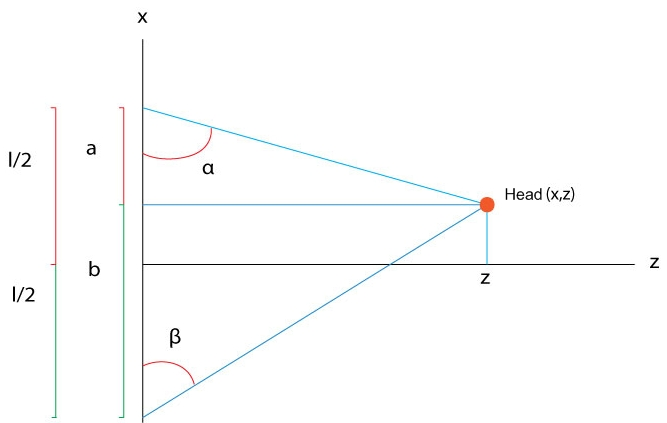
\includegraphics[width=0.45\textwidth]{graphics/Figur_2_sensorer_english.jpg}
		\caption{Model for tracking}
	\end{figure}

We looked at the available technology for connecting a high definition camera to a PC and reading the images from it. We studied the properties of infrared light. We looked at and tested the Nintendo Wii game console and its Wiimotes. Lastly, potential areas of use for a solution was described.

	\begin{figure}[h]
		\centering
		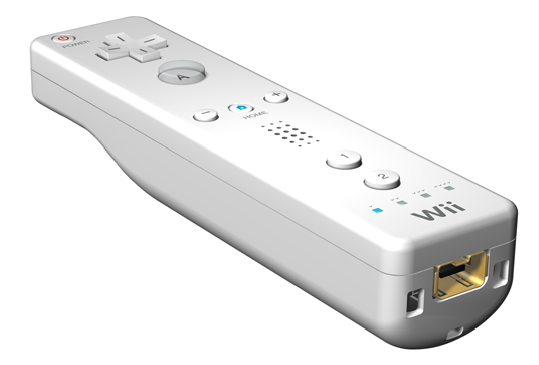
\includegraphics[width=0.25\textwidth]{graphics/wiimote2.png}
		\caption{A Nintento Wiimote controller}
	\end{figure}

\addtolength{\parskip}{0.05in}

\section{Requirements and design}

	A specification of the requirements was carefully crafted. It states that:
	
	\begin{itemize}
		\item The system should track the position of the user's head in three dimensions.
		\item The estimated position should be updated when the user moves.
		\item A 3D-scene should be shown in front of the user, and the viewpoint in the scene should be mapped to the head position.
		\item The price of the system should be below 10 000 NOK.
		\item The equipment the user needs to wear should be lighter than 300 grams.
	\end{itemize}
	
	The specification was the basis for the design of the solution. This design specifies how the components of the system is constructed and how they are connected. The components of the system make up a pipeline:
	
	\begin{figure}[h]
		\centering
		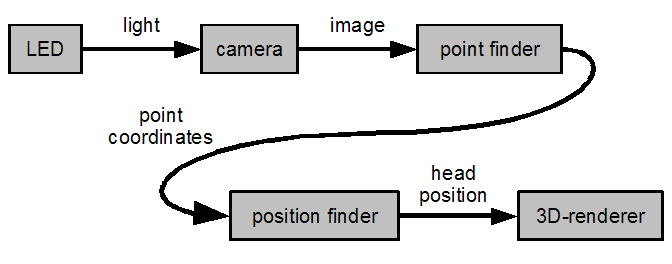
\includegraphics[width=0.45\textwidth]{graphics/main_design_english_narrow.png}
		\caption{The main design of the system}
	\end{figure}
	
	The LED-component is a set of infrared LEDs that are attached to the user's head. These transmit light that is captured by a high definition camera. The image from this camera is read by our point finder software that attempts to locate the coordinates of the bright dots in the image where the LEDs are. These coordinates are transferred to the position finder software which uses them to estimate the position of the user's head. This head position is then used by the 3D-renderer software to display a 3D-scene on a screen where the viewpoint is mapped to the head position.
	
\section{Implementation}

	The implementation was done by acquiring a Panasonic high definition digital camera and connecting this to a PC with an HDMI-card. In addition, a headset with infrared LEDs was constructed. For the software part, the point finder, posistion finder and 3D-renderer was written in Java with bindings to native machine code for the 3D-rendering part.
	
	\begin{figure}[h]
		\centering
		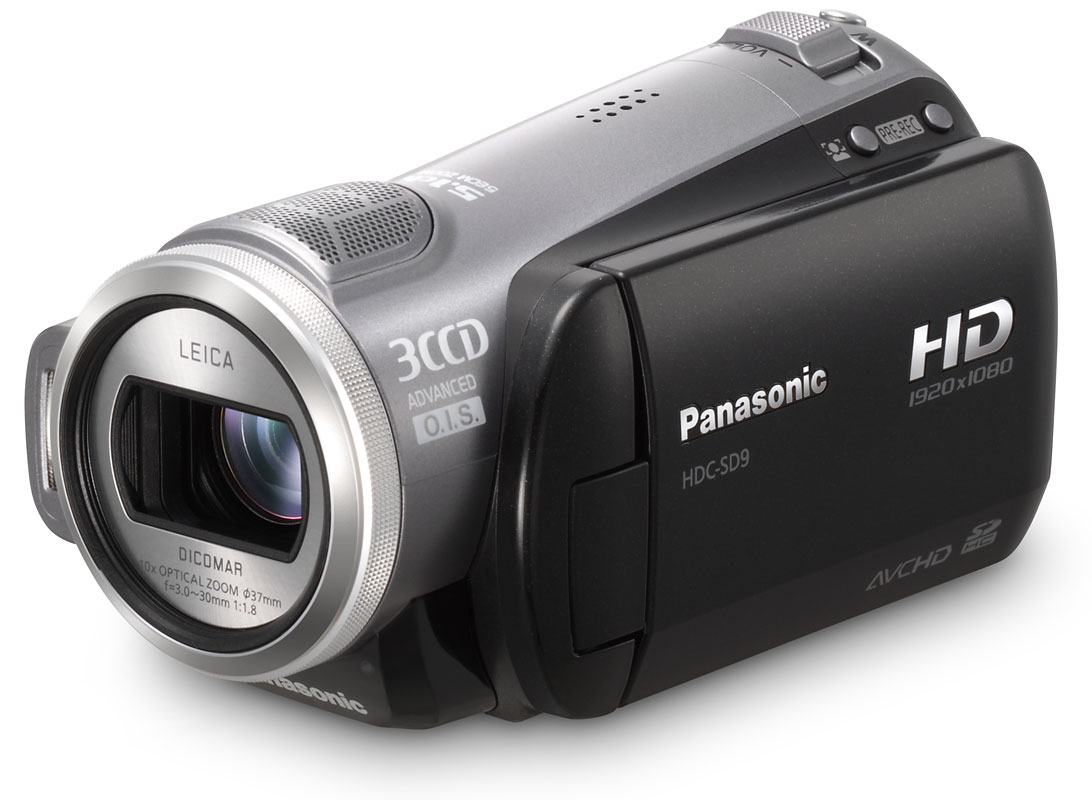
\includegraphics[width=0.3\textwidth]{graphics/hdcam.jpg}
		\caption{Panasonic HDC-SD9}
	\end{figure}

\section{The result}
	
	We ended up with an adaptive solution. In addition to using the high definition camera connected to a PC by HDMI, one can use a Nintendo Wiimote by wireless Bluetooth network. Even {\em two} Wiimotes can be used for improved tracking. The system follows the requirements and design specifications. It provides virtual reality by tracking the position of the user's head and displaying a 3D-scene on a screen in front of the user. The viewpoint in this scene is moved to match the position of the head. This creates the sensation of looking into a real room through the sceen.
	
	A head moves by rotation and translation, or yaw, pitch, roll, left/right, up/down or forward/back, which sums up to six degrees of freedom (6DOF). Head tracking refers to the estimation of rotation, translation or both, usually based on optical sensors like cameras and infrared lights. The system can be compared to the commercial TrackIR \cite{trackir} or the freely available FreeTrack \cite{freetrack}.

	The solution proposed here calculates head translation and thus provides 3DOF head tracking. This is sufficient since virtual reality, by accurate 3D perspective projection, is only dependant on head translation. However, depending on which mode the system is in, which can be either one optical sensor mode or two optical sensors mode, the user will still have 5DOF and 6DOF movement respectively. 
	
	Two demonstration applications showing the use of head tracking and accurate 3D perspective projection are included in the solution. The first demonstration application shows how an illusion of objects breaking the surface in the screen can be achieved using head tracking, giving a very immersive experience. The second demonstration is an equally or even more immersive game, where the player must avoid obstacles hurdled towards him, by ducking, jumping and dodging side-to-side.

\section{Conclusion}
	
	The hardware cost of the solution is below 10 000 NOK. It is easy to set up and use and provides a strong sensation of reality. Thus, we conclude that it is possible to create such an affordable and usable system for head tracking as in the problem statement.
	
\section{Acknowledgements}

	We would like to thank virtual reality village chief Egil Tj�land for an inspiring enthusiasm. Thorvald Natvig and Knut Bakke are to be thanked for their technical assistance. And the EiT learning assistants are appreciated for their guidance and facilitation.
	
\bibliographystyle{plain}
\bibliography{literature}

\end{document}